\section{Implementacija}

Prethodna poglavlja opisivala su metodu \emph{toon shading}-a te način implementacija koji se svodi na izradu \emph{shader} programa. No sam \emph{shader} program, izvodi se na grafičkoj kartici. U ovom poglavlju opisuje se sučelje koje je izrađeno za potrebe rada, koje krajnjem korisniku omogućava izmjenu modela i \emph{shader} programa. Opisuje se način implemntacije, te interakcija sa grafičkom karticom korištenjem \emph{three.js} biblioteke za rad s WebGL-om.

Aplikacija je izrađena pomoću HTML5 tehnologije i \emph{JavaScrip} programskog jezika. Na taj način, omogućeno je izvršavanje neovisno o platformi na većini modernih internet preglednika, te uređajima koji podržavaju HTML5 \emph{canvas} element. Budući da mogućnost izvršavanja aplikacije ovisi o grafičkom procesoru i karakteristikama samoga uređaja, korištena je biblioteka \emph{modernizer}\footnote{https://modernizr.com/} za određivanje sklopovske podrške samoga uređaja na kojemu se aplikacija izvršava.

Aplikacija podržava statični prikaz modela te animaciju rotacijom modela oko svoje osi, kako bi se mogućnosti \emph{shader} korisničkoga programa mogle proučiti iz više kutova pod različitom rasvjetom. Izrađen je na način da se prilagođava veličini ekrana, kako bi se mogla izvršavati na uređajima raznih veličina. Korisničko sučelje prikazano je na slici \ref{fig:interface}.

\begin{figure}[H]
\centering\fbox{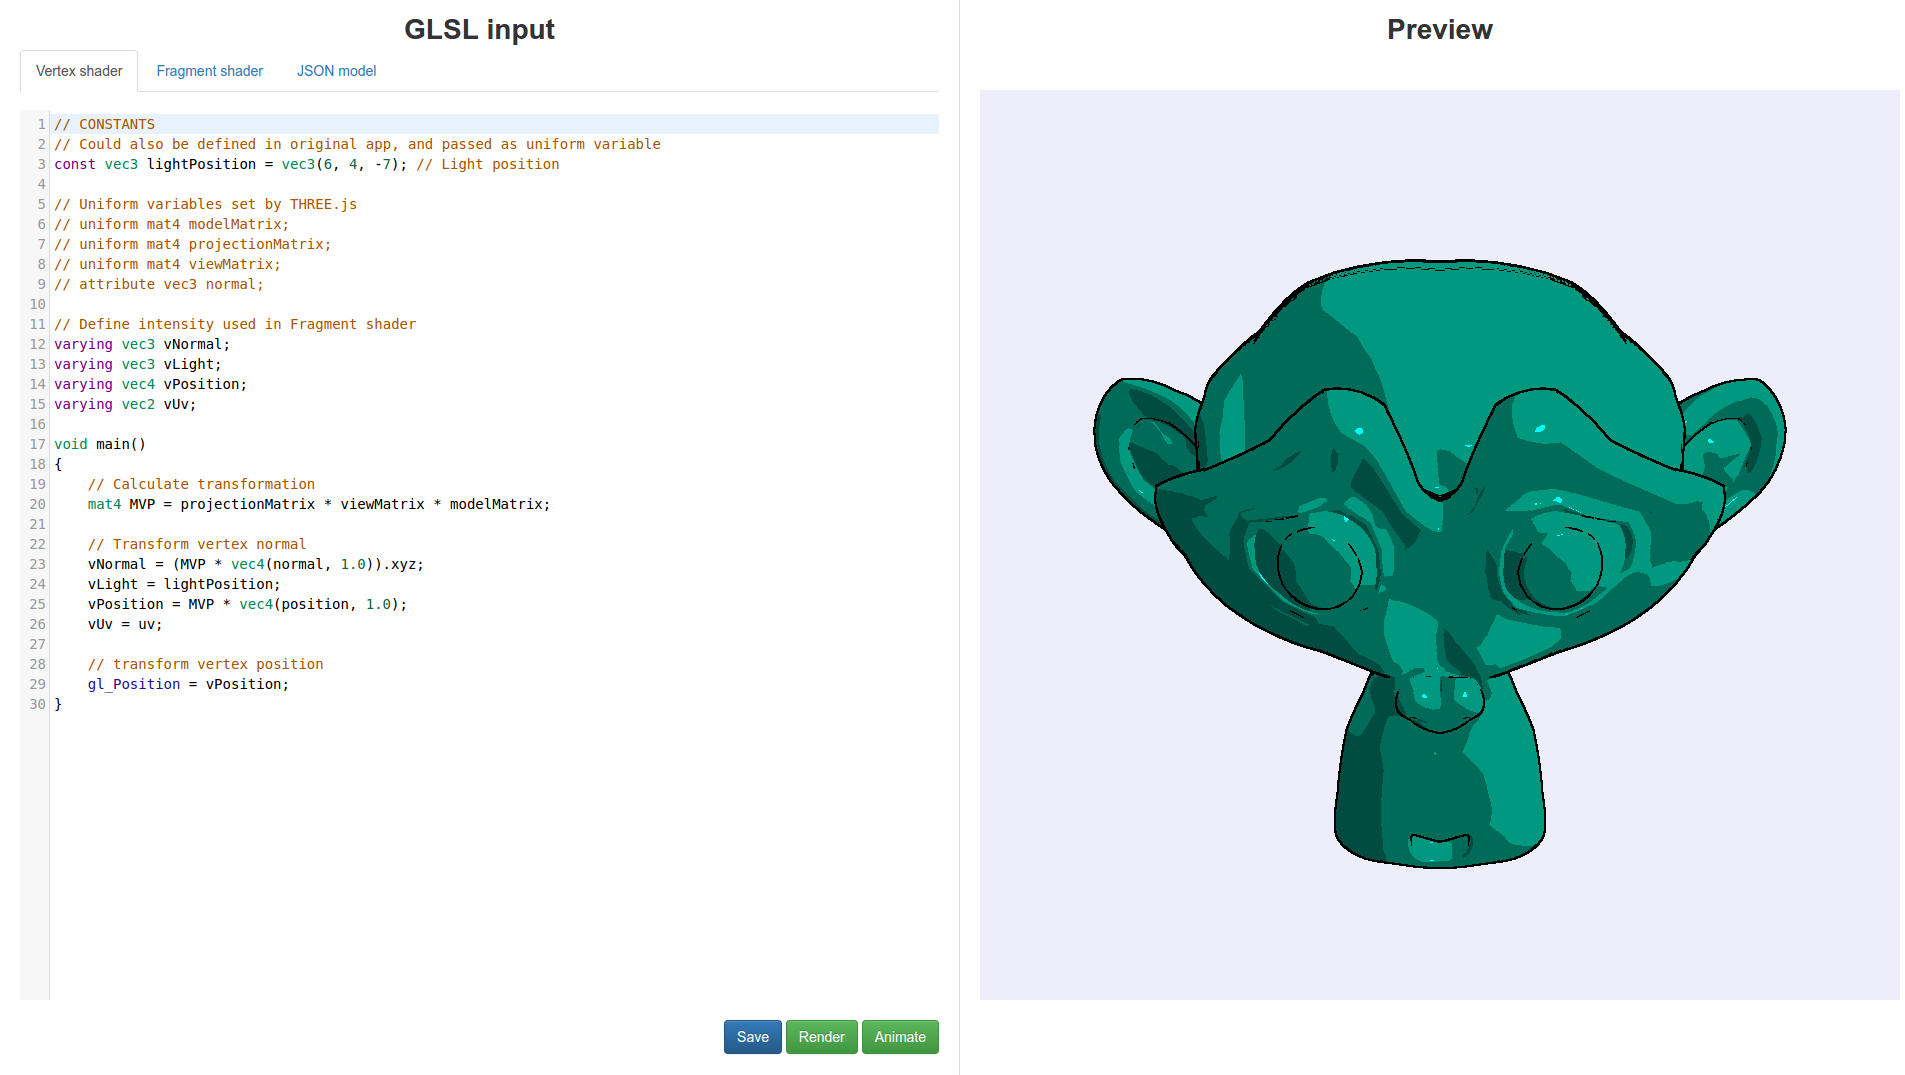
\includegraphics[scale=0.2]{interface.png}}
\caption{Korisničko sučelje aplikacije}
\label{fig:interface}
\end{figure}

\subsection{Korištenje \emph{three.js}-a}

\emph{Three.js} \cite{threejs-github} biblioteka napisana je u JavaScript programskom jeziku i služi za kreiranje i prikaz 3D sadržaja u internet preglednicima. Sama biblioteka omogućava krajnjem korisniku brži pristup grafičko kartici, te olakšava procese učitavanja i prijenosa modela. Također omogućava lakši rad sa korisničkim \emph{shader} programima.

Prva javno dostupna verzija biblioteke pojavila se početkom 2010.g. Od onda se razvija kao projekt otvorenoga koda pod \emph{MIT licencom}. Svoju popularnost počela je postizati godinu dana kasnije, kada je internet preglednik \emph{Firefox} razvio podršku za WebGL. Trenutno broji preko 600 suradnika koji su doprinijeli izvornom kodu.

\subsection{Učitavanje modela}

Aplikacija učitava modele u \emph{three.js JSON} formatu. Većina današnjih alata za 3D modeliranje podržava ovaj format nativno ili kroz dodatke koji se naknadno instaliraju na aplikaciju. Za potrebe ovoga rada korišten je programski alat \emph{Blender}\footnote{https://www.blender.org/}, pomoću kojega je u \emph{three.js JSON} formatu izvezena prilagođena verzija modela \emph{monkey} koji dolaz sa alatom, prikazan na slici \ref{fig:blender-monkey}.

\begin{figure}[H]
\centering\fbox{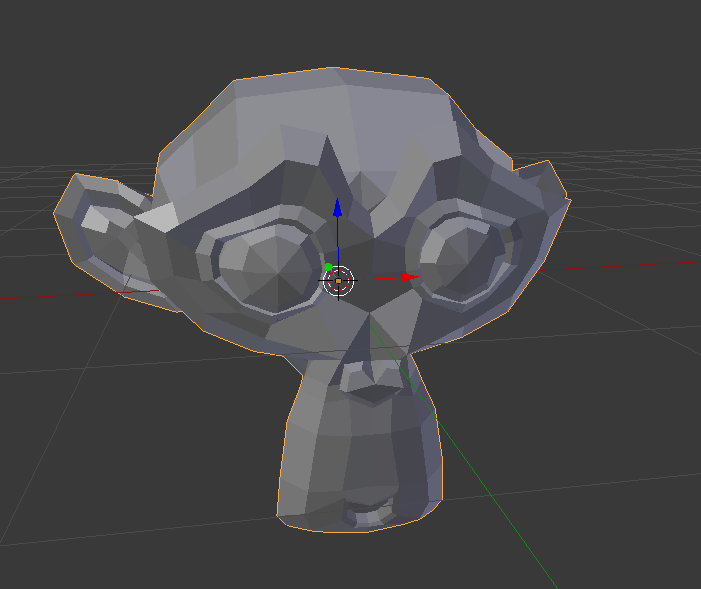
\includegraphics[scale=0.3]{blender_monkey.png}}
\caption{Osnovni \emph{Monkey} model iz alata \emph{Blender}}
\label{fig:blender-monkey}
\end{figure}

Unutar same aplikacije korišten je \emph{three.js} osnovni objekt \emph{THREE.JSONLoader} \footnote{http://threejs.org/docs/api/loaders/JSONLoader.html} koji je zadužen za kreiranje samoga modela na grafičkoj kartici preko ulazne datoteke. \emph{THREE.JSONLoader} objektu se prosljeđuje sadržaj same datoteke u tekstualnom formatu.

Korisničko sučelje aplikacije učitava sadržaj datoteke na način da korisnik sadržaj mora unijeti u za to predviđeno mjesto (na kartici \emph{JSON model}) te potvrditi svoj unos pritiskom na tipku \emph{Save}. U tome trenutku aplikacija će korisnički unos spremiti u lokalno spremište internet preglednika, kako korisnik ne bi morao ponavljati ovu radnju prilikom sljedećega korištenja aplikacije. Prilikom uspješnoga spremanja izmjena korisnik dobiva obavijest kao što je prikazano na slici \ref{fig:interface-save}.

\begin{figure}[H]
\centering\fbox{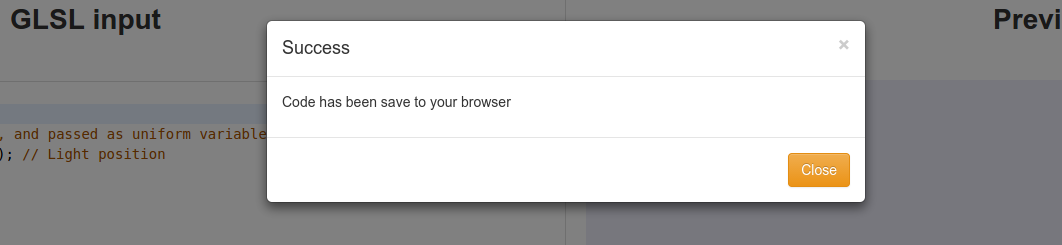
\includegraphics[scale=0.3]{interface_success.png}}
\caption{Obavijest krajnjem korisniku nakon spremanja izmjena}
\label{fig:interface-save}
\end{figure}

Učitani model potom se prosljeđuje objektu \emph{THREE.Mesh} \footnote{http://threejs.org/docs/\#Reference/Objects/Mesh}, koji služi za daljnju interakciju modela i aplikacije. Budući da se sam model nalazi na grafičkoj kartici, a ne u radnoj memoriji računala, \emph{THREE.Mesh} kao povratnu informaciju aplikaciji vraća identifikacijsku oznaku modela, koja ga jednoznačno označava u memoriji grafičke kartice. Na taj način vrši se komunikacija i interakcija između modela i ostatka aplikacije.

\subsection{Učitavanje korisničkoga \emph{shader} programa}

Slično kao i učitavanja samoga modela, vrši se i učitavanje \emph{shader} korisničkoga programa. Na karticama \emph{Vertex shader} i \emph{Fragment shader} predviđen je unos korisničkih programa. Aplikacija podržava naglašavanje sintakse, kako bi omogućila krajnjem korisniku olakšani rad. Sam unos vrši se na način da korisnik mora unijeti izvorni kod \emph{shader} korisničkoga programa u za to predviđena mjesta. Kao i prilikom unosa modela, nakon unosa programskog koda, korisnik mora potvrditi svoj unos pritiskom na tipku \emph{Save}, kako bi se programski kod spremio u lokalno spremište internet preglednika za naknadnu upotrebu. Prilikom uspješnoga spremanja izmjena korisnik dobiva obavijest kao što je prikazano na slici \ref{fig:interface-save}.

Korištenjem \emph{three.js} osnovnog objekta \emph{THREE.ShaderMaterial} \footnote{http://threejs.org/docs/api/materials/ShaderMaterial.html} kreira se \emph{materijal} na kojemu se vrši sjenčanje korisničkim programom. Prilikom stvaranja materijala, objekt prima nekoliko ulaznih parametara:

\begin{itemize}
\item \textbf{vertexShader:} Izvorni kod \emph{vertex shader} korisničkog programa koji je prethodno unesen
\item \textbf{fragmentShader:} Izvorni kod \emph{fragmentShader} korisničkog programa koji je prethodno unesen
\item \textbf{uniforms:} \emph{Uniform} varijable koje če biti proslijeđene \emph{shader} korisničkom programu prilikom izvršavanja.
\end{itemize}

Za potrebe ove aplikacije korišteno je nekoliko \emph{uniform} varijabli, od kojih je najbitnija \emph{pass} koja označava indeks sloja koji se trenutno obrađuje, kako je opisano u poglavlju \ref{sec:shading} ovoga rada. Izuzev \emph{pass} varijable, \emph{shader} programu potrebno je proslijediti i reference na dvije teksture koje su mu potrebne za rad, kao što je kasnije pojašnjeno u poglavlju \ref{sec:multipass-rendering}, koje programu omogućuju izvršavanje u više iteracija.

Sam objekt \emph{THREE.ShaderMaterial} zadužen je prijenos izvornoga koda na grafičku karticu, te njegovo kompajliranje. Uslijed uspješnog prijenosa, objekt \emph{THREE.ShaderMaterial} nam vraća jednoznačnu referencu na izvršni program u memoriji grafičke kartice koji se dalje koristi za interakciju s ostatkom aplikacije. No u koliko prijenos nije bio uspješan, odnosno došlo je do pogreške (najčešće uslijed pogreške u izvornom kodu korisičkog \emph{shader}-a), \emph{three.js} biblioteka nas o tome obavještava putem konzole internet preglednik.

Budući da konzolni prozor internet preglednika nije odmah dostupno, poželjno ga je otvoriti prilikom rada s aplikacijom, kako bi pravovremeno uočili pogreške. Također, aplikacija izrađena za potrebe ovoga rada i sama otkriva određene pogreške, te o tome obavještava krajnjega korisnika kako bi se pogreška uočila i prije otvaranja konzolnog prozora. Jedan takav primjer prikazan je na slici \ref{fig:interface-error}. gdje je došlo do pogreške prilikom učitavanja modela.

\begin{figure}[H]
\centering\fbox{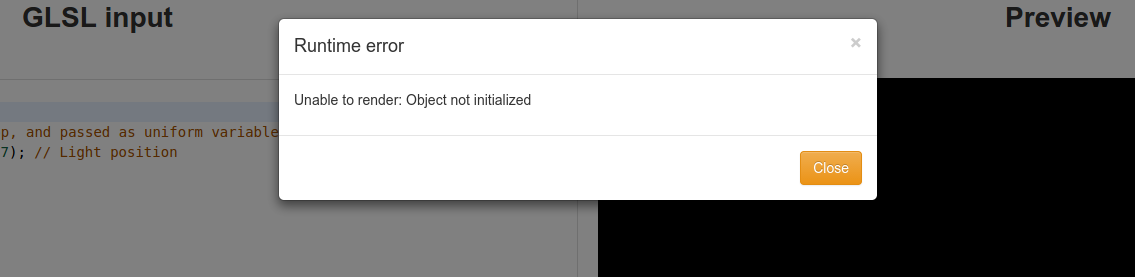
\includegraphics[scale=0.3]{interface_error.png}}
\caption{Obavijest o pogrešci prilikom izvođenja aplikacije}
\label{fig:interface-error}
\end{figure}

\subsection{Korištenje više slojeva}
\label{sec:multipass-rendering}

Kao što je prethodno opisano u poglavlju \ref{sec:shading}, ova implementacija \emph{toon shader} načina sjenčanja zahtjeva više iteracija za postizanje željenoga efekta. Budući da grafički cjevovod, kako je opisano u poglavlju \ref{sec:opengl-pipeline}, radi na razini \emph{pixel}-a i fragmenata, pojedina iteracija nema pristup cjelovitoj slici, niti je moguće rezultat u konačnici vratiti na ulaz cjevovoda. Iz toga razlika, korištene su dvije teksture kako je prethodno opisano.

Teksture u \emph{OpenGL}-u su slike koje se mogu \emph{nalijepiti} na materijal pojedinog objekta na sceni. Sam \emph{fragment shader} zadužen je za mapiranje teksture na objekt. Iz toga razloga, teksture su naprijed učitane u memoriju grafičke kartice, te su u potpunosti dostupne svakom fragmentu u \emph{fragment shader} korisničkom programu. Dostupnost cijele slike omogućava pretraživanje susjedstva \emph{pixel}-a opisanoga u poglavlju \ref{sec:edge-detection}, za svaki fragment pojedinačno.

Kako bi omogućili \emph{shader} korisničkom programu dostupnost rezultata iz prethodnih iteracija, rezultat prve dvije iteracija sprema se izravno u odgovarajuću teksturu u memoriji grafičke kartice, umjesto da se prikazuje korisniku na ekran. Na posljednjoj iteraciji, \emph{shader} korisnički program ima pristup objema teksturama (iscrtanoj dubini modela prikazanoj na slici \ref{fig:monkey-depth} i osjenčanoj verziji modela prikazanoj na slici \ref{fig:monkey-toon}), te je taj korak zadužen za stapanje rezultata i konačni prikaz na korisnikov ekran, odnosno \emph{HTML5 canvas} element na grafičkom sučelju krajnjega korisnika.

\subsection{Pokretanje aplikacije}

Nakon što je korisnik unio izvorni kod \emph{shader} programa te nakon što je unio 3D model, potrebno je odabrati način prikaza modela:

\begin{itemize}
\item \textbf{Statični prikaz:} Pritiskom na tipku \emph{Redner} pokreće se statični prikaz osjenčanoga modela gdje je model okrenut izravno prema kameri. Dobiva se rezultat kao što je prikazan na slici \ref{fig:monkey-final}.

\item \textbf{Animirani prikaz:} Pritiskom na tipku \emph{Animate} pokreće sa animacija modela, na način da se model okreće oko svoje osi. Na taj način omogućava se pregled iz raznih kuteva, kao što je prikazano na slici \ref{fig:monkey-toonshaded}.
\end{itemize}

Korisničko sučelje omogućava kontinuirane izmjene na \emph{shader} korisničkom programu i 3D modelu. Nakon napravljenih izmjena, potrebno je ponovno odabrati način rada, te će izmjene biti odmah vidljive. Ovdje je potrebno napomenuti kako \emph{three.js}\footnote{Verzija 73, koja je korištena za potrebe ovoga rada} ne podržava izmjene svih komponenti na sceni. Iz tog razloga, za veće izmjene u radu \emph{shader} korisničkoga programa, potrebno je spremiti izmjene i osvježiti prozor internet preglednika, kako bi se aplikacija nanovo inicijalizirala, te kako bi se svi resursi nanovo učitali u memoriju grafičke kratice.